% =====================================================================
%  AetherGrid AI - Data Flow Diagrams (Level 0, Level 1, Level 2)
%  Compile: pdflatex aethergrid_dfd.tex
% =====================================================================
\documentclass[11pt,a4paper]{article}
\usepackage[T1]{fontenc}
\usepackage[utf8]{inputenc}
\usepackage{mathpazo}
\usepackage{helvet}
\usepackage[margin=1.8cm]{geometry}
\usepackage{xcolor}
\usepackage{amsmath}
\usepackage{caption}
\usepackage{float}
\usepackage{tikz}
\usetikzlibrary{arrows.meta,positioning,calc}

\definecolor{navy}{HTML}{2F5233}
\definecolor{lightfill}{HTML}{F4EFE5}
\captionsetup{font=small,labelfont={bf,sf,color=navy},skip=8pt}

\tikzset{
  % Process bubbles
  proc0/.style={draw=navy,thick,fill=lightfill,circle,minimum size=2.8cm,
                align=center,inner sep=1pt},
  proc/.style={draw=navy,thick,fill=lightfill,circle,minimum size=2.0cm,
               align=center,inner sep=1pt},
  proc2/.style={draw=navy,thick,fill=lightfill,circle,minimum size=2.0cm,
                align=center,inner sep=1pt},
  % External entities
  ext/.style={draw=navy,thick,fill=white,minimum width=2.8cm,
              minimum height=1.0cm,align=center,font=\small\sffamily},
  % Boundary terminators (Level 2)
  term/.style={draw=navy,thick,fill=white,minimum width=2.6cm,
               minimum height=0.88cm,align=center,font=\scriptsize\sffamily,
               rounded corners=2pt},
  % Open-ended Gane & Sarson data store
  datastore/.style={
    draw=none,fill=white,minimum width=2.6cm,minimum height=0.72cm,
    align=center,font=\scriptsize\sffamily,inner sep=3pt,
    append after command={
      \pgfextra{
        \draw[navy,thick] (\tikzlastnode.north east) -- (\tikzlastnode.north west)
                       -- (\tikzlastnode.south west) -- (\tikzlastnode.south east);
      }
    }
  },
  % Connectors & labels
  fl/.style={-{Stealth[length=2.4mm,width=1.4mm]},navy,thick},
  fllb/.style={font=\scriptsize\sffamily,fill=white,inner sep=1.5pt,align=center}
}

\begin{document}

% =====================================================================
%  LEVEL 0 - CONTEXT DIAGRAM
% =====================================================================
\begin{figure}[H]
\centering
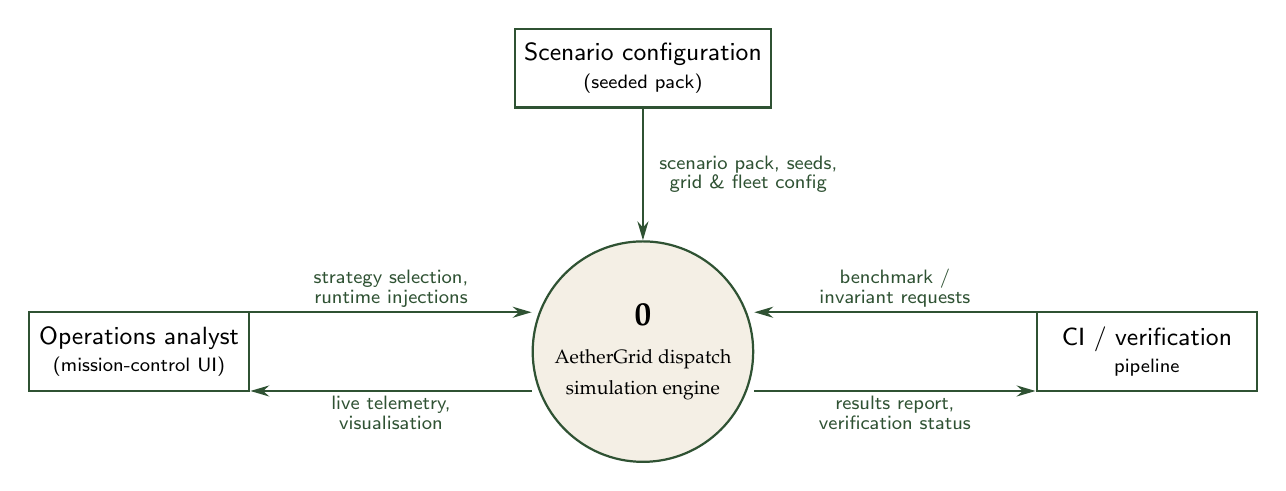
\begin{tikzpicture}
  \node[proc0] (p0) at (0,0)
    {\textbf{\large 0}\\[2pt]{\scriptsize AetherGrid dispatch}\\[-1pt]{\scriptsize simulation engine}};

  \node[ext] (e1) at (-6.4,0) {Operations analyst\\[-1pt]{\scriptsize (mission-control UI)}};
  \node[ext] (e2) at (6.4,0)  {CI / verification\\[-1pt]{\scriptsize pipeline}};
  \node[ext] (e3) at (0,3.6)  {Scenario configuration\\[-1pt]{\scriptsize (seeded pack)}};

  % E3 -> P0
  \draw[fl] (e3.south) -- node[midway,right=4pt,fllb] {scenario pack, seeds,\\[-1pt]grid \& fleet config} (p0.north);

  % E1 <-> P0
  \draw[fl] ([yshift=5mm]e1.east) -- node[midway,above,fllb] {strategy selection,\\[-1pt]runtime injections} ([yshift=5mm]p0.west);
  \draw[fl] ([yshift=-5mm]p0.west) -- node[midway,below,fllb] {live telemetry,\\[-1pt]visualisation} ([yshift=-5mm]e1.east);

  % E2 <-> P0
  \draw[fl] ([yshift=5mm]e2.west) -- node[midway,above,fllb] {benchmark /\\[-1pt]invariant requests} ([yshift=5mm]p0.east);
  \draw[fl] ([yshift=-5mm]p0.east) -- node[midway,below,fllb] {results report,\\[-1pt]verification status} ([yshift=-5mm]e2.west);
\end{tikzpicture}
\caption{\textbf{Level 0 (Context Diagram).} Global system boundary with bidirectional operational and verification corridors.}
\label{fig:dfd0}
\end{figure}

\clearpage

% =====================================================================
%  LEVEL 1 - SYSTEM DECOMPOSITION (CALIBRATED ZERO-COLLISION LAYOUT)
% =====================================================================
\begin{figure}[H]
\centering
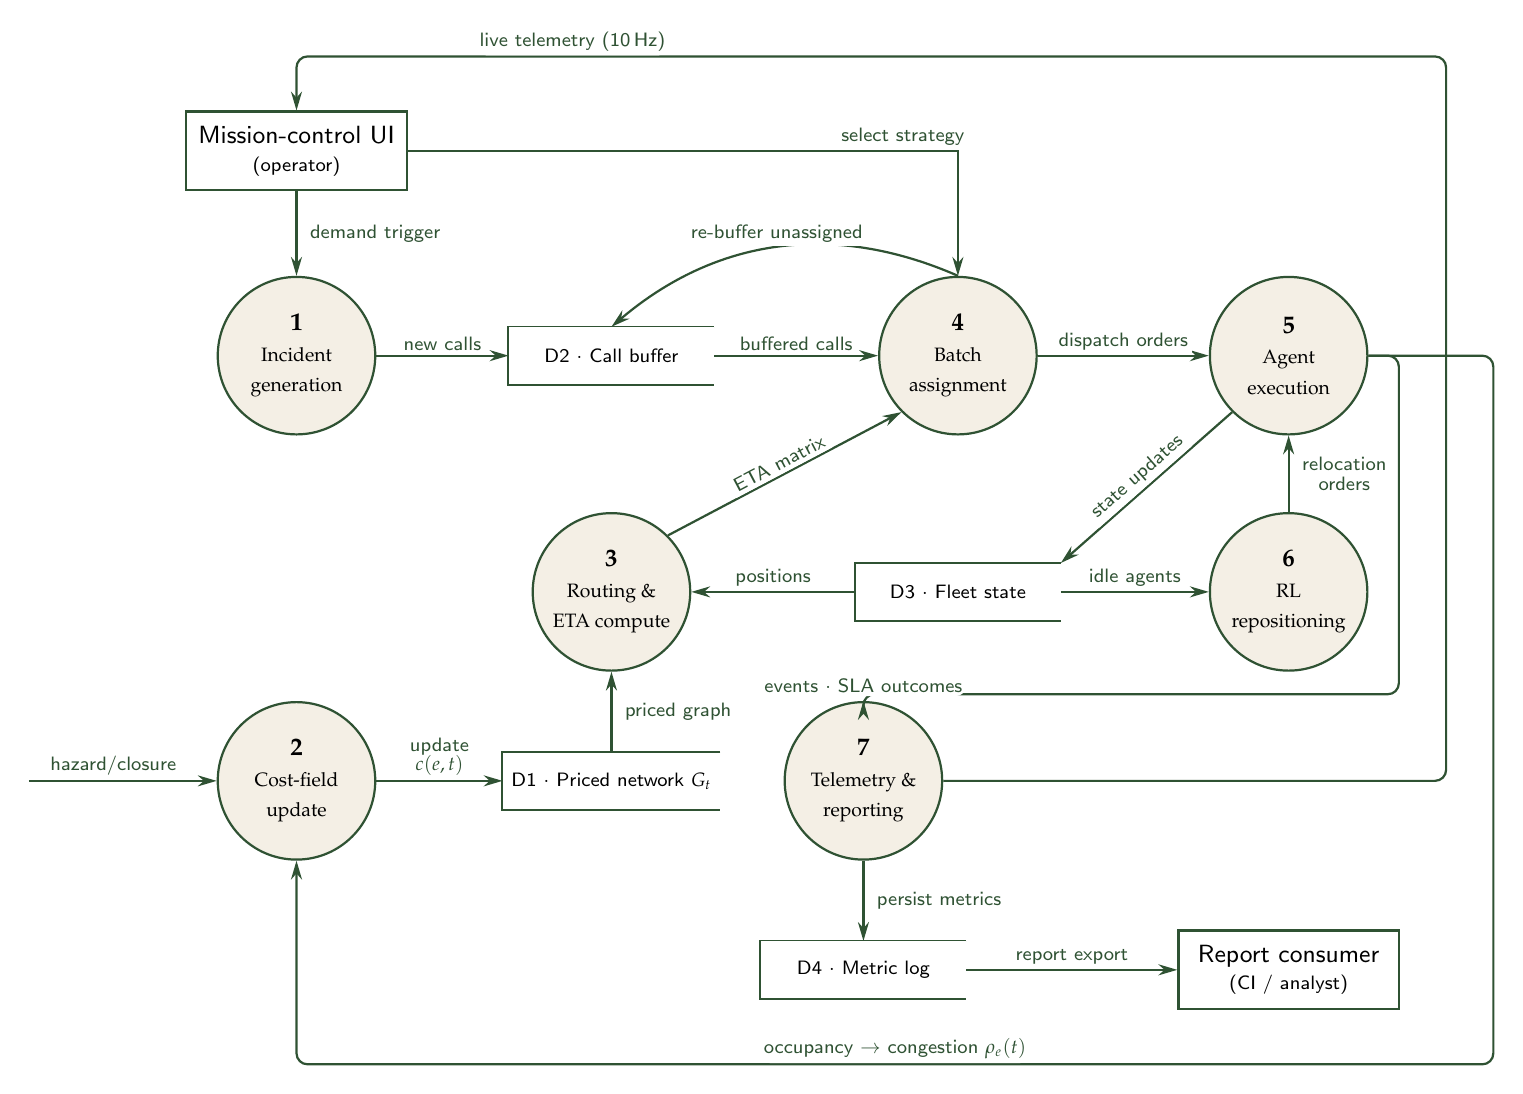
\begin{tikzpicture}
  % Row 4: y = 9.2 (Operator)
  % Row 3: y = 6.6 (Primary pipeline: P1, D2, P4, P5)
  % Row 2: y = 3.6 (Compute & Fleet:   P3, D3, P6)
  % Row 1: y = 1.2 (Cost & Reporting:  P2, D1, P7)
  % Row 0: y = -1.2 (Metrics & CI:     D4, E2)

  % --- Nodes ---
  \node[ext] (e1) at (1.8,9.2) {Mission-control UI\\[-1pt]{\scriptsize (operator)}};

  \node[proc] (p1) at (1.8,6.6) {\textbf{\small 1}\\[-1pt]{\scriptsize Incident}\\[-1pt]{\scriptsize generation}};
  \node[proc] (p2) at (1.8,1.2) {\textbf{\small 2}\\[-1pt]{\scriptsize Cost-field}\\[-1pt]{\scriptsize update}};

  \node[datastore] (d2) at (5.8,6.6) {D2 $\cdot$ Call buffer};
  \node[proc]      (p3) at (5.8,3.6) {\textbf{\small 3}\\[-1pt]{\scriptsize Routing \&}\\[-1pt]{\scriptsize ETA compute}};
  \node[datastore] (d1) at (5.8,1.2) {D1 $\cdot$ Priced network $G_t$};

  \node[proc]      (p4) at (10.2,6.6){\textbf{\small 4}\\[-1pt]{\scriptsize Batch}\\[-1pt]{\scriptsize assignment}};
  \node[datastore] (d3) at (10.2,3.6){D3 $\cdot$ Fleet state};
  \node[proc]      (p7) at (9.0,1.2)  {\textbf{\small 7}\\[-1pt]{\scriptsize Telemetry \&}\\[-1pt]{\scriptsize reporting}};

  \node[proc]      (p5) at (14.4,6.6){\textbf{\small 5}\\[-1pt]{\scriptsize Agent}\\[-1pt]{\scriptsize execution}};
  \node[proc]      (p6) at (14.4,3.6){\textbf{\small 6}\\[-1pt]{\scriptsize RL}\\[-1pt]{\scriptsize repositioning}};

  \node[datastore] (d4) at (9.0,-1.2) {D4 $\cdot$ Metric log};
  \node[ext]       (e2) at (14.4,-1.2){Report consumer\\[-1pt]{\scriptsize (CI / analyst)}};

  % --- Row 3: Main Forward Pipeline (y = 6.6) ---
  \draw[fl] (e1.south) -- node[midway,right=3pt,fllb] {demand trigger} (p1.north);
  \draw[fl] (p1.east)  -- node[midway,above,fllb] {new calls} (d2.west);
  \draw[fl] (d2.east)  -- node[midway,above,fllb] {buffered calls} (p4.west);
  \draw[fl] (p4.east)  -- node[midway,above,fllb] {dispatch orders} (p5.west);

  % Re-buffer loop (P4 -> D2) & Strategy input (E1 -> P4)
  \draw[fl] (p4.north) to[bend right=32] node[midway,above,fllb] {re-buffer unassigned} (d2.north);
  \draw[fl] (e1.east)  -| node[pos=0.45,above,fllb] {select strategy} (p4.north);

  % --- Row 2: ETA Matrix & State Updates ---
  \draw[fl] (d1.north) -- node[midway,right=3pt,fllb] {priced graph} (p3.south);
  \draw[fl] (d3.west)  -- node[midway,above,fllb] {positions} (p3.east);
  \draw[fl] (p3.north east) -- node[midway,above,sloped,fllb] {ETA matrix} (p4.south west);
  \draw[fl] (p5.south west) -- node[midway,above,sloped,fllb] {state updates} (d3.north east);

  % Process 6 (Repositioning)
  \draw[fl] (d3.east)  -- node[midway,above,fllb] {idle agents} (p6.west);
  \draw[fl] (p6.north) -- node[midway,right=3pt,fllb] {relocation\\[-1pt]orders} (p5.south);

  % --- Row 1: Cost-Field Updates & Hazard Origin (Guaranteed Clear Runway) ---
  \draw[fl] (-1.6,1.2) -- node[pos=0.45,above,fllb] {hazard/closure} (p2.west);
  \draw[fl] (p2.east)  -- node[midway,above,fllb] {update\\[-1pt]$c(e,t)$} (d1.west);

  % --- Row 0: Metrics Persistence & Report Export (Guaranteed 2.7 cm Runway) ---
  \draw[fl] (p7.south) -- node[midway,right=3pt,fllb] {persist metrics} (d4.north);
  \draw[fl] (d4.east)  -- node[midway,above,fllb] {report export} (e2.west);

  % --- Outer Multi-Track Corridors ---
  % Track 1 (x = 15.8): Events to Telemetry
  \draw[fl,rounded corners=4pt] (p5.east) -- (15.8,6.6) -- (15.8,2.3) -- (9.0,2.3)
        -- node[pos=0.45,above,fllb] {events $\cdot$ SLA outcomes} (p7.north);

  % Track 2 (x = 16.4): Telemetry Loop to UI
  \draw[fl,rounded corners=4pt] (p7.east) -- (16.4,1.2) -- (16.4,10.4)
        -- node[pos=0.76,above,fllb] {live telemetry (10\,Hz)} (1.8,10.4)
        -- (e1.north);

  % Track 3 (x = 17.0, y = -2.4): Congestion Loop (Clear of E2 and D4 by >7 mm)
  \draw[fl,rounded corners=4pt] (p5.east) -- (17.0,6.6) -- (17.0,-2.4)
        -- node[pos=0.5,above,fllb] {occupancy $\rightarrow$ congestion $\rho_e(t)$} (1.8,-2.4)
        -- (p2.south);
\end{tikzpicture}
\caption{\textbf{Level 1.} Complete operational flow decomposition with isolated feedback paths and non-intersecting event corridors.}
\label{fig:dfd1}
\end{figure}

\clearpage

% =====================================================================
%  LEVEL 2a - PROCESS 4 (BATCH ASSIGNMENT)
% =====================================================================
\begin{figure}[H]
\centering
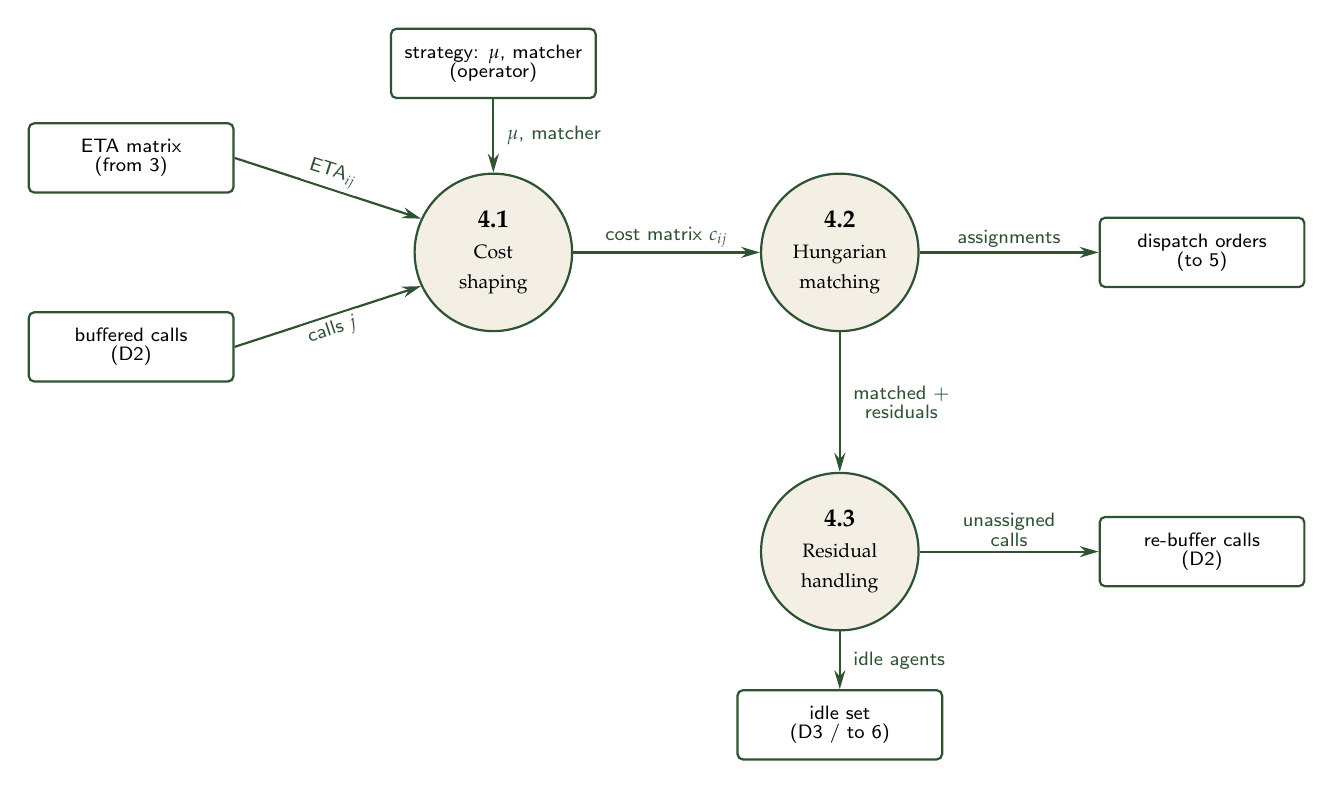
\begin{tikzpicture}
  % Core Process Pipeline
  \node[proc2] (p41) at (3.4,3.2) {\textbf{\small4.1}\\[-1pt]{\scriptsize Cost}\\[-1pt]{\scriptsize shaping}};
  \node[proc2] (p42) at (7.8,3.2) {\textbf{\small4.2}\\[-1pt]{\scriptsize Hungarian}\\[-1pt]{\scriptsize matching}};
  \node[proc2] (p43) at (7.8,-0.6){\textbf{\small4.3}\\[-1pt]{\scriptsize Residual}\\[-1pt]{\scriptsize handling}};

  % Boundary Terminators
  \node[term] (tstrat) at (3.4,5.6)  {strategy: $\mu$, matcher\\[-1pt]{\scriptsize (operator)}};
  \node[term] (teta)   at (-1.2,4.4) {ETA matrix\\[-1pt]{\scriptsize (from 3)}};
  \node[term] (tcalls) at (-1.2,2.0) {buffered calls\\[-1pt]{\scriptsize (D2)}};

  \node[term] (tdisp)  at (12.4,3.2) {dispatch orders\\[-1pt]{\scriptsize (to 5)}};
  \node[term] (trebuf) at (12.4,-0.6){re-buffer calls\\[-1pt]{\scriptsize (D2)}};
  \node[term] (tidle)  at (7.8,-2.8) {idle set\\[-1pt]{\scriptsize (D3 / to 6)}};

  % Inputs to 4.1
  \draw[fl] (tstrat.south) -- node[midway,right=3pt,fllb] {$\mu$, matcher} (p41.north);
  \draw[fl] (teta.east)   -- node[midway,above,sloped,fllb] {ETA$_{ij}$} (p41.155);
  \draw[fl] (tcalls.east) -- node[midway,below,sloped,fllb] {calls $j$} (p41.205);

  % Internal Pipeline
  \draw[fl] (p41.east) -- node[midway,above,fllb] {cost matrix $c_{ij}$} (p42.west);
  \draw[fl] (p42.south) -- node[midway,right=3pt,fllb] {matched +\\[-1pt]residuals} (p43.north);
  \draw[fl] (p42.east) -- node[midway,above,fllb] {assignments} (tdisp.west);

  % Outputs from 4.3
  \draw[fl] (p43.east) -- node[midway,above,fllb] {unassigned\\[-1pt]calls} (trebuf.west);
  \draw[fl] (p43.south) -- node[midway,right=3pt,fllb] {idle agents} (tidle.north);
\end{tikzpicture}
\caption{\textbf{Level 2 --- Process 4 (Batch Assignment).} Deconstruction of cost shaping, matching, and residual set partitioning.}
\label{fig:dfd2a}
\end{figure}

\vspace{0.6cm}

% =====================================================================
%  LEVEL 2b - PROCESS 5 (AGENT EXECUTION)
% =====================================================================
\begin{figure}[H]
\centering
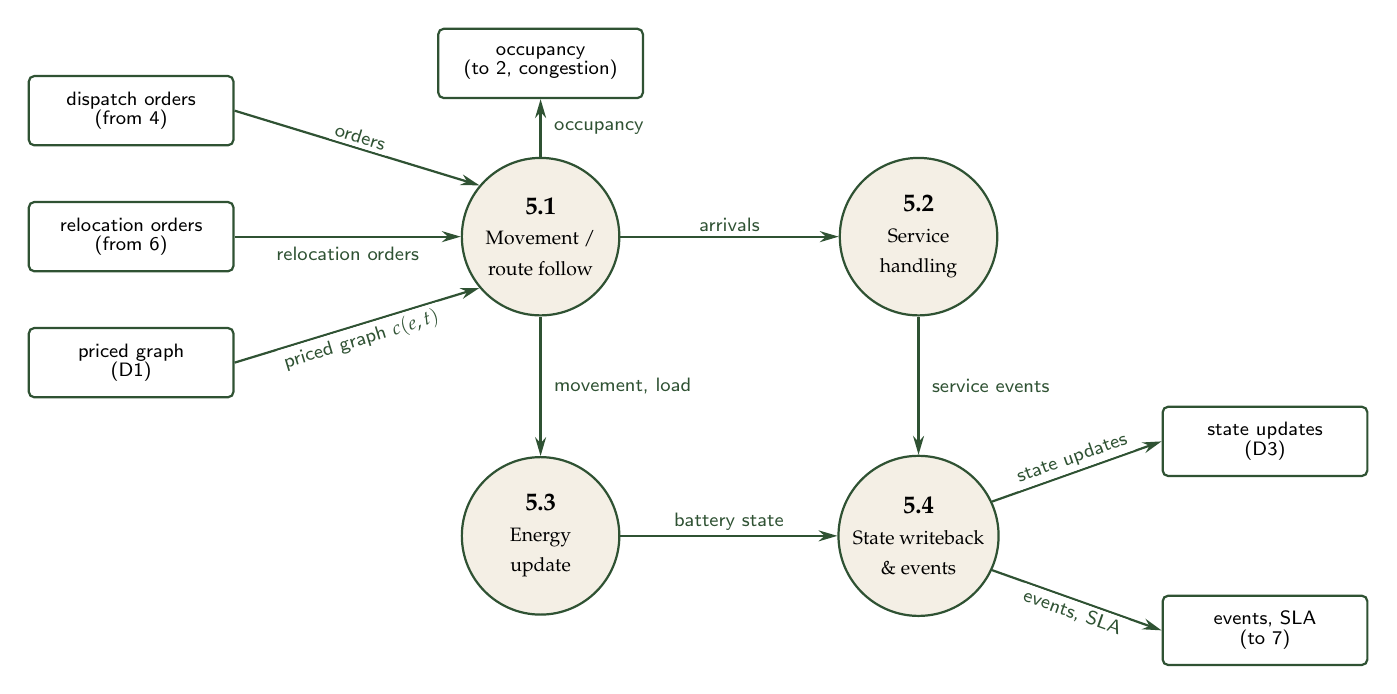
\begin{tikzpicture}
  % Core 2x2 Process Grid
  \node[proc2] (p51) at (3.8,3.2) {\textbf{\small5.1}\\[-1pt]{\scriptsize Movement /}\\[-1pt]{\scriptsize route follow}};
  \node[proc2] (p52) at (8.6,3.2) {\textbf{\small5.2}\\[-1pt]{\scriptsize Service}\\[-1pt]{\scriptsize handling}};
  \node[proc2] (p53) at (3.8,-0.6){\textbf{\small5.3}\\[-1pt]{\scriptsize Energy}\\[-1pt]{\scriptsize update}};
  \node[proc2] (p54) at (8.6,-0.6){\textbf{\small5.4}\\[-1pt]{\scriptsize State writeback}\\[-1pt]{\scriptsize \& events}};

  % Boundary Terminators
  \node[term] (tdisp)  at (-1.4,4.8) {dispatch orders\\[-1pt]{\scriptsize (from 4)}};
  \node[term] (treloc) at (-1.4,3.2) {relocation orders\\[-1pt]{\scriptsize (from 6)}};
  \node[term] (tgraph) at (-1.4,1.6) {priced graph\\[-1pt]{\scriptsize (D1)}};

  \node[term] (tp2)    at (3.8,5.4)  {occupancy\\[-1pt]{\scriptsize (to 2, congestion)}};
  \node[term] (td3)    at (13.0,0.6) {state updates\\[-1pt]{\scriptsize (D3)}};
  \node[term] (tp7)    at (13.0,-1.8){events, SLA\\[-1pt]{\scriptsize (to 7)}};

  % Inputs to 5.1
  \draw[fl] (tdisp.east)  -- node[midway,above,sloped,fllb] {orders} (p51.140);
  \draw[fl] (treloc.east) -- node[midway,below=2pt,fllb] {relocation orders} (p51.west);
  \draw[fl] (tgraph.east) -- node[midway,below,sloped,fllb] {priced graph $c(e,t)$} (p51.220);

  % Congestion exit straight north
  \draw[fl] (p51.north) -- node[midway,right=3pt,fllb] {occupancy} (tp2.south);

  % Internal Process Pipeline
  \draw[fl] (p51.east)  -- node[midway,above,fllb] {arrivals} (p52.west);
  \draw[fl] (p51.south) -- node[midway,right=3pt,fllb] {movement, load} (p53.north);
  \draw[fl] (p52.south) -- node[midway,right=3pt,fllb] {service events} (p54.north);
  \draw[fl] (p53.east)  -- node[midway,above,fllb] {battery state} (p54.west);

  % Outputs from 5.4
  \draw[fl] (p54.25)  -- node[midway,above,sloped,fllb] {state updates} (td3.west);
  \draw[fl] (p54.335) -- node[midway,below,sloped,fllb] {events, SLA} (tp7.west);
\end{tikzpicture}
\caption{\textbf{Level 2 --- Process 5 (Agent Execution).} Internal agent simulation pipeline with dedicated entry/exit corridors and decoupled congestion telemetry.}
\label{fig:dfd2b}
\end{figure}

\end{document}
